\documentclass[10pt,a4paper]{ctexart}
\usepackage[utf8]{inputenc}
\usepackage{amsmath}
\usepackage{amsfonts}
\usepackage{amssymb}
\usepackage{graphicx}
\usepackage{xcolor}
\usepackage{bm}
\author{吴秉哲}
\title{数值分析上机报告}
\begin{document}
\maketitle
这学期每次的上机报告都按如下格式编写:

每份报告分为几个章节,每个章节分别介绍上机作业中的一题,其中每个
题目又分为以下几个部分:
\begin{enumerate}
\item 问题提出及相关背景知识
\item 问题的理论分析及解决方案
\item 程序的部分设计思路与细节
\item 计算成果与分析
\item 本次上机的反思
\end{enumerate}
每个题目中要求回答的问题均蕴含在问题的理论分析与计算成果分析两部分

在程序方面,都是由C++编写完成(其中用到了自己编写的库:矩阵(Matrix),向量(Vector),以及数值代数的相关算法(linear)),在linux下由g++编译。数据方面
一般使用matlab可视化处理,少部分使用了python。
\section{第一章第二题}
\subsection{问题提出及相关背景知识}
提出如下形式的积分:
\[I_n=\int_{0}^{1}\dfrac{x^n}{x+5}dx \ \ \ n=0,1,2\cdots \]
题目要求计算$I_1,I_2,\cdots I_{20}$的值
\subsection{问题的理论分析及解决方案}
记$f_n(x)=\dfrac{x^n}{x+5}$,则当$x\in [0,1)$时,有:\[\lim_{n\rightarrow \infty}f_n(x)=0\]
且上述的收敛是一致的,则进一步有:
\[\lim_{n\rightarrow \infty}I_n=0\]
由上式可以知道,如果算法设计合理,那么当n足够大的时候,程序计算
出来的$\left|I_n-I_{n-1}\right|$足够小。
下面在理论上推导程序需要的递推关系,首先推导题目中要求的向前递推公式,易知:
\begin{equation*}
\begin{split}
\dfrac{x^n}{x+5}&=\dfrac{x}{x+5}x^{n-1}\\
& =\dfrac{x+5-5}{x+5}x^{n-1}\\
& =x^{n-1}-5\dfrac{x^{n-1}}{x+5}
\end{split}
\end{equation*}
由上面推导可以得到:
\begin{equation}
\begin{split}
I_0&=\int_{0}^{1}\dfrac{1}{x+5}=ln1.2\\
I_n&=-5I_{n-1}+\int_{0}^{1}x^{n-1}\\
& =-5I_{n-1}+\dfrac{1}{n}
\end{split}
\end{equation}
(1)式即为题目要求推导的递推关系式,在上式中,形式上是由前一项计算后一项的值,于是,将其称为向前递推公式。

但从(1)式来看,当n增大时,$I_{n-1}$与$\dfrac{1}{n}$会逐渐靠近,这样用(1)计算积分时,会出现两个大小接近的
数相减,会损失精度,会有大的误差。另一方面,设计算的初始误差为$E_0$(这是由于计算机进行实数运算肯定会有一定的误差),将第n步的误差记为$E_n$即有
$E_n=I_n-\overline{I_n}$,而$\overline{I_n}$表示第n步计算解,则由上面的递推公式得\textcolor{red}{$E_n=(-1)^n(5!)E_0$}.由此可以知道,即使初始误差很小,但误差任然被不断的放大,导致后面的计算结果严重失真,这是一个不稳定的算法。后面的计算结果也印证了这一点。
于是,我们可以预知用这个递推式计算时,计算结果会很不合理。到这里,我们可以根据递推式的特点,设计另外一种算法如下:
首先对上面推导得出的递推式变形,得到向后递推公式:
\[I_{n-1}=-\dfrac{1}{5}I_n+\dfrac{1}{5n}\]
上面的公式是教材题目要求的递推公式的变形,它的主要特点是由$I_n$
计算$I_{n-1}$,初始值$I_{20}$我们可以通过梯形法得一个近似值,
实验表明,虽然初始误差相比第一种方法较大,但是随着计算的进行,舍入误差被不断的缩小。可以证明这是一个稳定的数值算法。
下面我们编写程序来验证
我们的两种方法。
\subsection{程序设计的思路与细节}
本题的编写很简单,只要按照(1)式,直接编写程序即可。本题编写了一个由前项$I_{n-1}$计算$I_n$的子函数。
\subsection{计算成果与分析}
为了使程序的结果有对比,我还使用了Matlab中自带的数值积分的计算函数计算题目所给积分的值。由于篇幅,只列出了题目要求的第一种方法的计算结果。
下面列出在double与float(C语言)环境下,程序的计算结果:
\par
\centerline{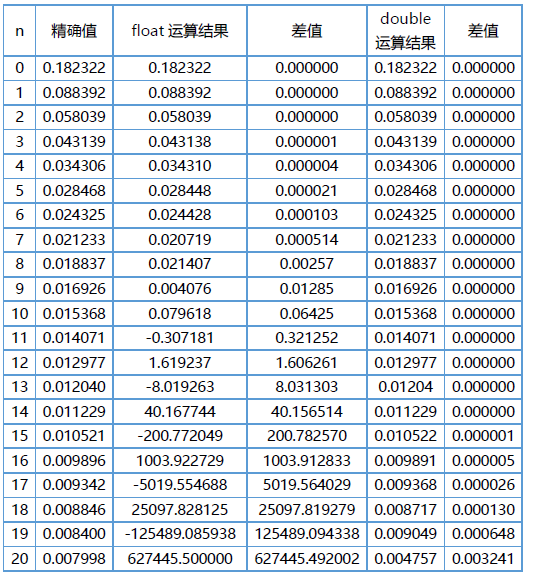
\includegraphics{计算结果.png}}
\par
从上述结果明显可以看出,递推公式(1)的计算误差很明显,尤其是在float精度下,从n=8时,$I_n$与真实值开始有明显差距。并且随着n的增大,误差也在变大。这与我们的理论分析相符合。因此我们可以回答题目的第二问:这个递推公式在电脑上的计算结果并不合理,原因见上面的理论分析。而第二种方法的计算结果,和我们理论分析一样,随着n的增大,计算的值与精确值也越来越接近。
\subsection{本次上机反思}
从这个题目的例子,我们知道很多在数学理论上很合理的结果,在数值上并不可靠,这是由于在电脑上,实数的运算并不遵循数学的规则,任何运算都会有误差,而有些不当操作会使误差变大,在设计算法时,思维不要局限在通常数学推导的范围,比如这个题,我们一般都会首先考虑向前递推,而不是更合理的向后递推,要对我们解决的实际问题进行充分的分析,然后设计数值稳定的算法,这样才能很好的解决问题。
\section {第二章第二题}
\subsection{问题提出及相关背景知识}
\begin{enumerate}
\item 问题提出

本体要求使用不同的插值方法(等距节点的newton,非等距节点的Lagrange插值,等距节点的分段线性,等距节点的Hermite,三次自然样条插值)
对Runge函数$R(x)=\dfrac{1}{1+x^2}$在区间$[-5,5]$进行插值逼近。最后得出不同的计算结果,从而对比各种方法的优劣。
\item 问题的背景知识

本题中的Runge函数,在使用等距节点上的高次插值时,会出现Runge现象:插值多项式在区间端点附件会出现震荡,严重偏离真实值。
产生这种现象的原因从复函数角度来看,是由于R(z)在$z=\pm i$处有奇性。

由此可见本题的目的就是让我们在实验中验证这种现象的存在,以及提出不同的插值方法来克服这种现象。
\end{enumerate}
\subsection{问题的理论分析及解决方案}
首先,由于上述Runge现象的存在,我们通常使用的等距高次插值就失效了,其次出了
上述的Runge现象外,等距高次插值方法的数值稳定性很差(详见教材P28)这诱导
我们从两个方向去改良方法,其一是将等距变为非等距,其二是将方法将高次变为分段低次插值。
基于这两种思路,我们就可以从题目中提到的方法去实验了。
\subsection{程序设计的思路与细节}
本次作业编写了一个关于多项式插值的一个库interpolation。将本次一些细节列在下面:
\begin{enumerate}
\item 编写Newton插值,需要写一个计算高阶差商的子函数,在这次上机中我采用等式$f[x_0,x_1,\cdots,x_m]=\sum\limits_{i=0}^{m}\dfrac{f(x_i)}{
\prod\limits_{j=0,j\neq i}^{m}(x_i-x_j)}$进行计算。也可以使用递归的方法编写。
\item 
在使用分段低次插值的算法时,首先需要确定x所在的区间$[x_i,x_{i+1}]$,我选择二分法进行搜索

\item 
注意到相应的分段插值,只需使用二分法确定x所在区间$[x_i,x_{i+1}]$后,在相应区间使用两点插值即可,
这个特点可以减少我们的工作量

\item 
在实现三次样条插值时,需要解一个线性方程组,只需注意到系数矩阵为三对角矩阵,且严格对家占优。于是,可以
通过追赶法和SOR迭代法求解。在本次上机中,我选取了追赶法。


\end{enumerate}
\subsection{计算成果与分析}
在上机中,首先在c++中将输出定向到一个文件,然后将文件的数据在matlab中绘图,下面分别列出各种方法与精确值的对比图象:
\par
\centerline{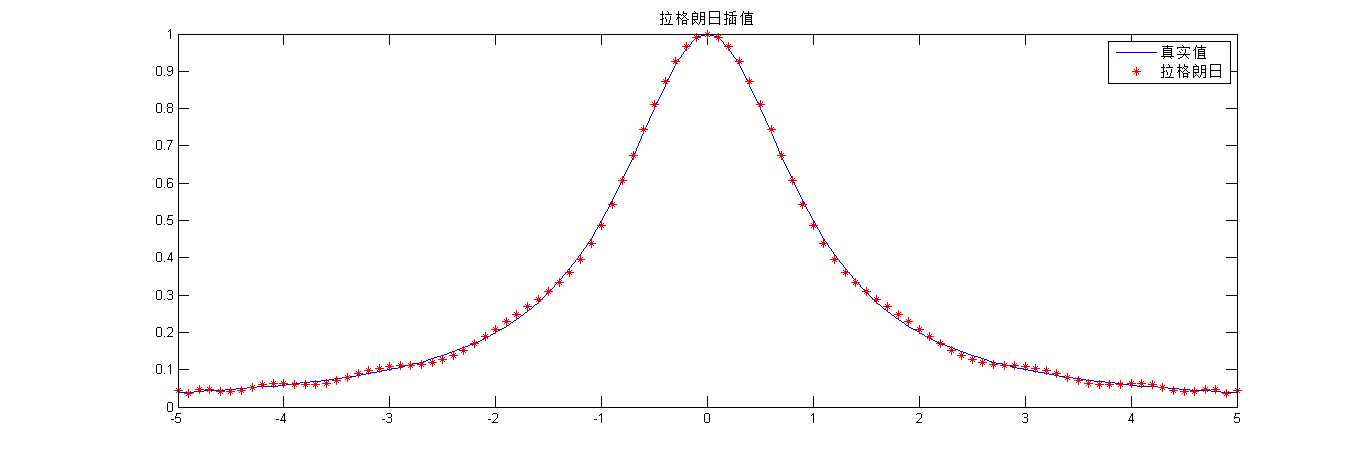
\includegraphics[height=5cm,width=18cm]{Lagrange.png}}
\centerline{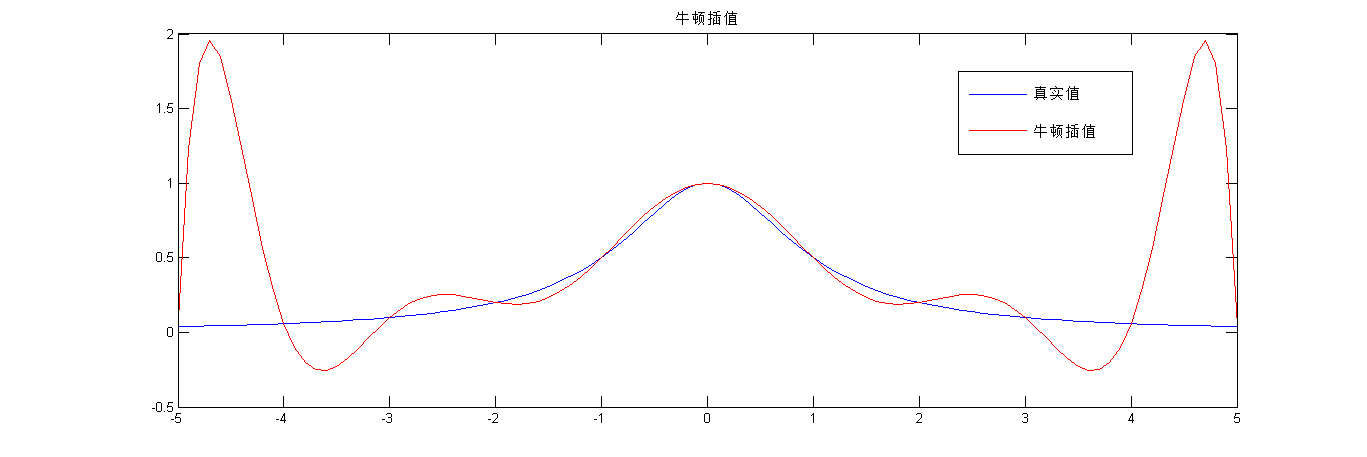
\includegraphics[height=5cm,width=18cm]{newton.png}}
\centerline{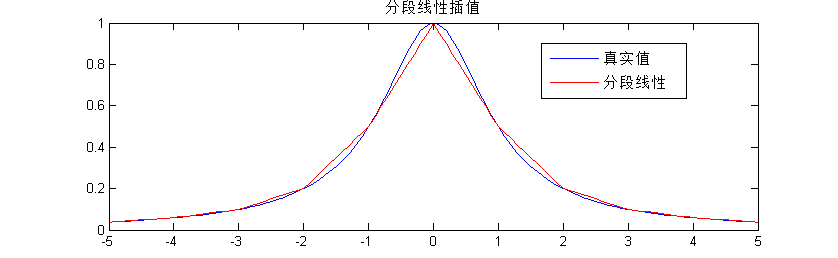
\includegraphics[height=5cm,width=18cm]{分段线性插值.png}}
\centerline{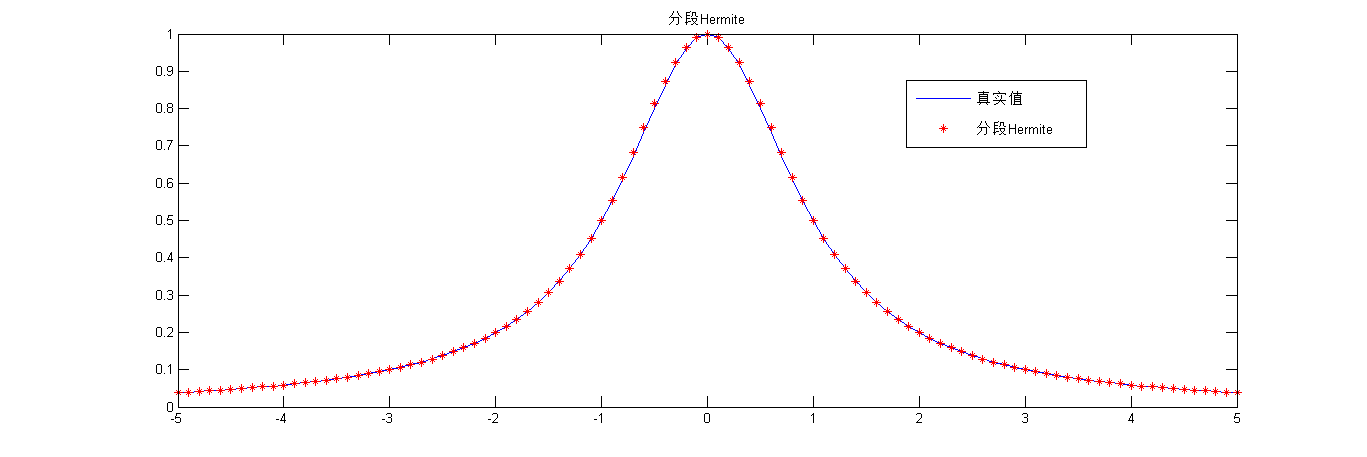
\includegraphics[height=5cm,width=18cm]{Hermite.png}}
\centerline{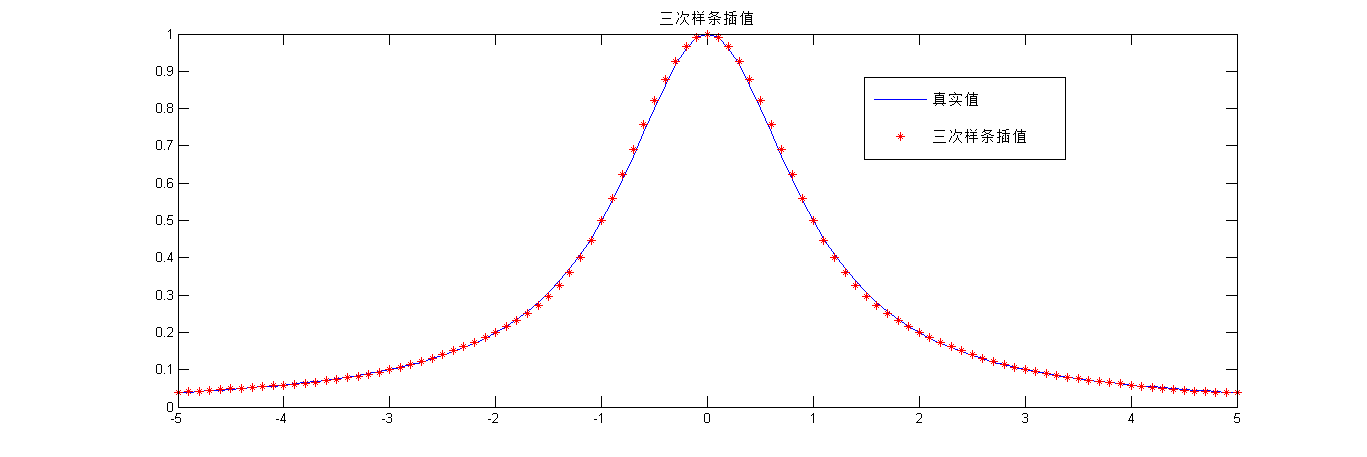
\includegraphics[height=5cm,width=18cm]{三次样条.png}}
\par
由上面的图像以及程序运行的结果可以得到这样一些特点:
\begin{enumerate}
\item 由牛顿插值所得到的图像,可以看出的确存在理论分析上的Runge现象
\item
相对于等距的牛顿插值,非等距的拉格朗日插值并没有出现Runge现象,已经可以得到与真实函数曲线相近的图像了,
但仔细观察数据,还是发现有一定的误差
\item 
分段线性插值所得到的结果不是特别好,有明显的误差,以及分段线性所得的曲线并不光滑,不能满足实际应用的一些要求
\item 
综合各种因素(数据,效果,算法实现的难易)来看,分段Hermite与三次自然样条插值所得到的结果比较好,其中
三次自然样条插值所得的曲线更加光滑
\item
从数据分析,在双精度环境下,分段Hermite插值与三次样条插值的精度基本达到了$10^{-3}$(在区间分为10等分下),
进一步细分区间可以得到更好的拟合曲线
\item 
综合上面的几幅图象,可以观察出当插值曲线的曲线变陡时,导数的绝对值值变大时,拟合的误差明显变大,这也与理论上分析出的截断误差表达式相符合。
\end{enumerate}
\subsection{本次上机反思}
这次上机总结了上机中遇到的问题
\begin{enumerate}
\item 在本次上机发现,选择合适的插值点,使用非等距的高次插值
也会得到不错的效果,所以在以后实际应用中,我们需要提前在理论上分析,然后得到合理的插值点,会起到事半功倍的效果
\item 在编写三次样条插值时,需要编写程序求解三对角方程,在这次上机中,多次由于边界条件处理不当,出现了程序的逻辑错误,所以以后在编写复杂的程序时,需要事先想清楚,然后再手动推算,这样会大大地提高程序的准确性。
\item 
这次的上机程序的流程比较清楚,先写好伪码,再上机实习,难度不大,出错的几率也较小
\item 
由于自己是为了编写数值算法的一些程序,自己学习了C++,对OOP编程的思想理解得不是很熟悉,在总结时,发现可以将插值的算法写一个类,这样可以大大的提高代码的重复可用性
\item 
在本次上机编写程序之前,在理论上进行了详细的分析,程序运行结果与理论上分析的大部分特点符合,也进一步印证了程序的正确性。所以在编写这种数值的算法之前
一定要进行数学理论分析,这样既可以保证程序的逻辑正确,也可以提高自己对算法的认识。
\item 
具体到本次的上机作业,综合各种因素,我认为三次样条插值方法是性价比最高的方法,在应用中应该是最有效的方法之一。
\item 
本次上机还有一些收获:虽然在这个题目中,通过使用非等距插值有效的
消除了振荡现象,但是实验表明,对于一般的非等距高次插值,振荡还是不能避免,为了验证这一点,我将插值点用C++的随机数生成函数生成,最后得到的结果还是存在严重的振荡现象。这要求我们在实际应用中,尽量使用分段低次插值。
\end{enumerate}

综上,就是本次上机的所有内容
\end{document}